\iffalse
\documentclass[12pt]{article}
\usepackage{graphicx}
\usepackage{amsmath}
\usepackage{mathtools}
\usepackage{gensymb}
\usepackage[utf8]{inputenc}
\usepackage{float}
\newcommand{\mydet}[1]{\ensuremath{\begin{vmatrix}#1\end{vmatrix}}}
\providecommand{\brak}[1]{\ensuremath{\left(#1\right)}}
\providecommand{\norm}[1]{\left\lVert#1\right\rVert}
\newcommand{\solution}{\noindent \textbf{Solution: }}
\newcommand{\myvec}[1]{\ensuremath{\begin{pmatrix}#1\end{pmatrix}}}
\let\vec\mathbf

\begin{document}
\begin{center}
\textbf\large{CLASS-11 \\ CHAPTER-10 \\ STRAIGHT LINES}
\end{center}
\section*{Excercise 10.4}

\section*{Solution}
\fi
The given line can be expressed as
\begin{align}
\myvec{1&-7}\vec{x}&=-5\\
\myvec{3&1}\vec{x}&=0
\end{align}
The intersection of two lines is given by row reducing the augmented matrix
\begin{align}
\myvec{
1&-7&5\\
3&1&0
}
\xleftrightarrow[]{R_2=R_2-3R_1}
\myvec{
1&-7&5\\
0&22&-15
}\\\xleftrightarrow[]{R_2=\frac{R_2}{22}}
\myvec{
  1&-7&5\\[1pt]
0&1&-\frac{15}{22}
}
\xleftrightarrow[]{R_1={R_1}+7{R_2}}
\myvec{
1&0&\frac{5}{22}\\[1pt]
0&1&\frac{-15}{22}
}
\end{align}
yielding
\begin{align}
  \vec{P}&=\myvec{-\frac{5}{22}\\[1pt] \frac{15}{22}}
\end{align}
The normal vector of the desired 
line is 
\begin{equation}
    \vec{n}=\myvec{1\\0}
    \label{eq:chapters/11/10/4/6/normal}
\end{equation}
The desired equation is then given by 
\begin{align}
	\vec{n}^{\top}\myvec{\vec{x}-\vec{P}}&=0
	\\
\implies 
	\myvec{1&0}\vec{x}&=-\frac{5}{22}
\end{align}
See Fig. 
\ref{fig:chapters/11/10/4/6/Fig3}
\begin{figure}[!ht]
  \begin{center} 
      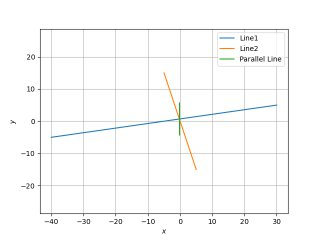
\includegraphics[width=\columnwidth]{chapters/11/10/4/6/figs/line_fig.png}
  \end{center}
\caption{}
\label{fig:chapters/11/10/4/6/Fig3}
\end{figure}
